\chapter{Introducción}
	\section{ESO y relación con Chile}
		\subsection{Antecedentes ESO en Chile}
			Chile, además de tener una gran cantidad de recursos naturales, cuenta con uno de los cielos más atractivos para la astronomía a nivel mundial, en especial aquel que cubre la zona desértica del norte de Chile (desierto de Atacama). El atractivo de este cielo se debe a la gran cantidad de noches despejadas ya que esta ubicado en zonas de altura con baja humedad que permiten una mayor captación de la luz. Por esta razón Chile alberga los telescopios más importantes y modernos del mundo y es un país anfitrión de la ESO.
			
			European Southern Observatory (ESO) es una reconocida organización intergubernamental de ciencia y tecnología. Su centro científico, técnico y administrativo está ubicado en Garching, Alemania. ESO cuenta con un programa de diseño y construcción de instalaciones para la observación astronómica que logra importantes avances en materia de la astronomía. Actualmente tiene tres instalaciones de observación, todas ellas en el desierto de Atacama: La Silla (\ref{fig:lasilla}), Paranal (\ref{fig:paranal}) y Chajnantor (\ref{fig:chajnantor}). Estas instalaciones nacen de un acuerdo entre el estado de Chile y la ESO, firmado en el año 1963. La primera instalación de telescopios en Chile corresponde al centro astronómico La Silla. Cuenta con telescopios ópticos de poca envergadura (diámetro máximo de 3.58 metros). Paranal, situado en la municipalidad de Tal-tal, es actualmente el centro de observación más importante del mundo el cual cuenta con seis telescopios, de los cuales cuatro de ellos son  UT (Unit Telescope) que poseen un espejo primario de un solo cuerpo con un diámetro de 8.2 metros que tienen la posibilidad de trabajar con los llamados AT (Auxiliar Telescope) los que permiten hacer espectrometría, simulando un “Espejo gigante”, de 200 metros de diámetro. El tercer y último sitio, ubicado en Chajnantor (en las cercanías de San Pedro de Atacama), está sobre los 5000 metros de altura, cuenta con un telescopio submilimetrico (APEX) y un telescopio conformado por un arreglo de antenas de 12 metros llamado Large Millimiter Array (ALMA) que es patrocinado por Chile y diferentes países de América del Norte, Asia del Este \cite{esoychile}.		
			\begin{figure}[t]
				\centering
				\begin{subfigure}[b]{0.45\textwidth}
					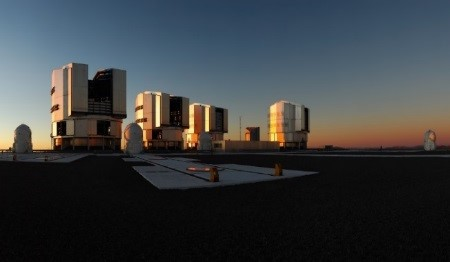
\includegraphics[width=	\textwidth,height=5cm]{paranal}
					\caption{Paranal}
					\label{fig:paranal}					
				\end{subfigure} 
				~~
				\begin{subfigure}[b]{0.45\textwidth}					
					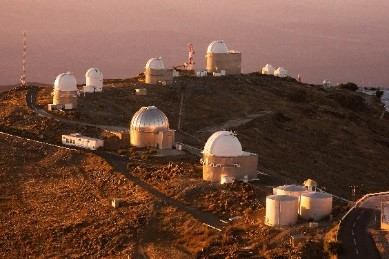
\includegraphics[width=\textwidth,height=5cm]{lasilla}
					\caption{La Silla}
					\label{fig:lasilla}					
			    \end{subfigure} \\
		    	\vspace{0.5cm}
		        \begin{subfigure}[b]{\textwidth}
					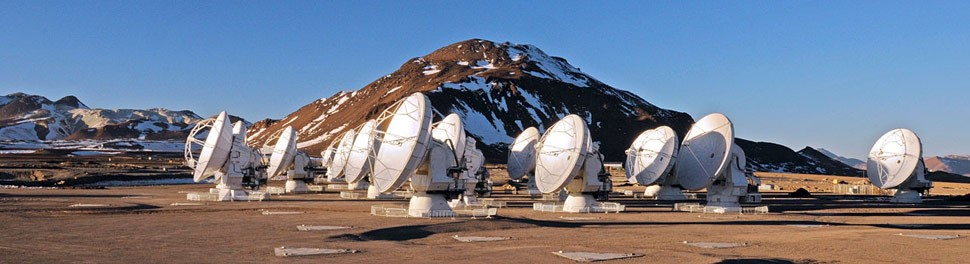
\includegraphics[width=\textwidth]{chajnantor}
					\caption{Chajnantor}
					\label{fig:chajnantor}					
				\end{subfigure}	
			\caption{Los tres centros astronómicos de ESO en Chile}	
			\label{observatorios}
			\end{figure}
		\subsection{Cerro Paranal}
			En el año 1988 Chile dona 72500 hectáreas a ESO para la construcción de un observatorio astronómico donde se toma la decisión de instalar un observatorio en cerro Paranal (región de Taltal), proyecto que se concluye el año 1998, año en el cual los telescopios entregan la primera observación gracias al telescopio UT1 (Antu). Es en el año 2001 cuando finalmente se construyen los 4 telescopios UT (figura \ref{fig:VLT}) y el año 2007 se construye el VLTI logrando emular espejos de gran diámetro gracias a los telescopios auxiliares (AT) y al VLTI tunnel, lugar donde a través de carros mecánicos se retrasa la llegada de la luz a los instrumentos. A esta tecnología se le conoce como interferometría.
			\begin{figure}
				\centering
				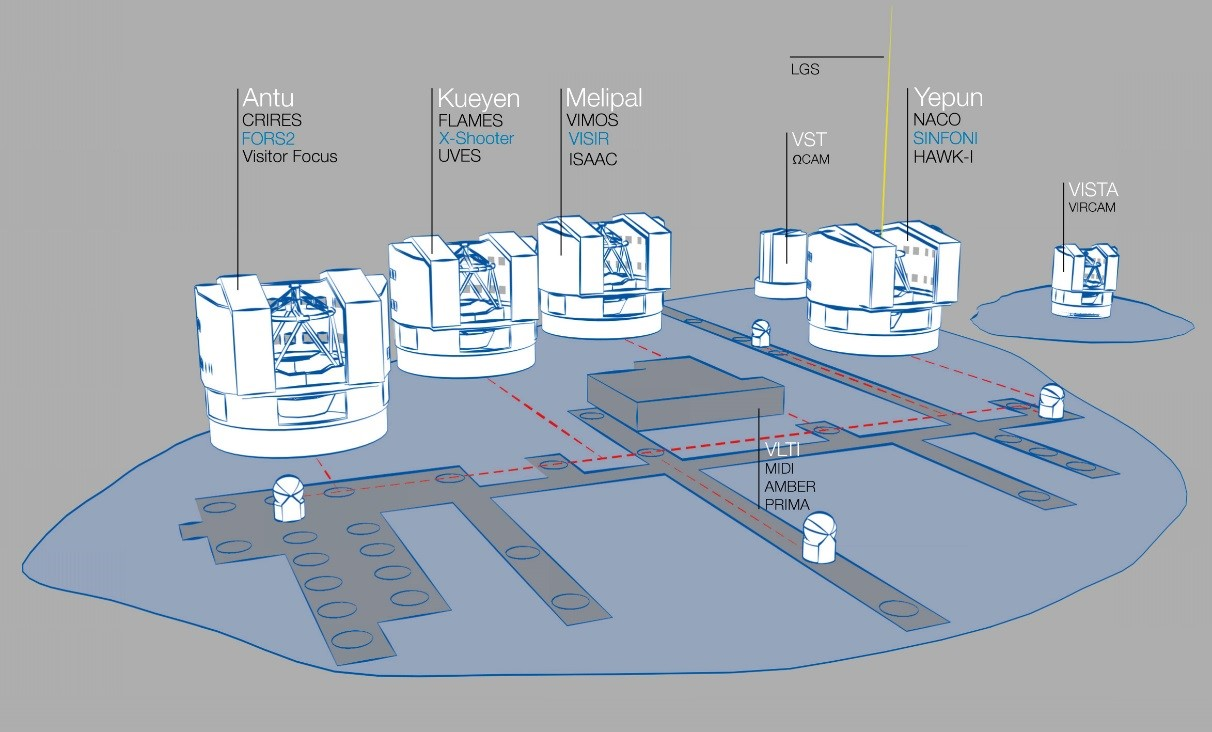
\includegraphics[width=0.8\textwidth]{vlt}
				\caption{Very Large Telescope (VLT) y sus instrumentos}
				\label{fig:VLT}
			\end{figure}
			\newpage
			Además de los 4 Unit Telescope mas VLTI, Paranal cuenta con dos 	telescopios más, VST (figura \ref{fig:carina}) survey telescope y VISTA (figura \ref{fig:lallama}) (Visible and Infrared Survey Telescope for Astronomy). Ambos telescopios están diseñados como telescopios de rastreo, es decir, son capaces de fotografiar porciones de cielo mayores a los que son capaces los UT.
			
			
			\begin{figure}[H]
				\centering
				\begin{subfigure}[b]{0.45\textwidth}
					
\includegraphics[width=\textwidth,height=5cm]{carina}
					\caption{Nebulosa Carina (VST)}
					\label{fig:carina}
				\end{subfigure}			    
			    \begin{subfigure}[b]{0.45\textwidth}
			    	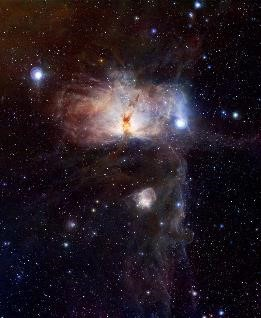
\includegraphics[width=\textwidth,height=5cm]{lallama}
			    	\caption{nebulosa La Llama (VISTA)}
			    	\label{fig:lallama}
			    \end{subfigure}
		    \caption{Imagenes capturadas por VST y Vista}
		    \label{fig:vstvistaimages}
		    \end{figure}
	    \subsection{Los telescopios UT (Unit Telescopes)}	    
	    	Los telescopios están constituidos por diferentes estructuras y sistemas que le permiten funcionar de manera eficiente (figura \ref{fig:UTorganigrama}). Destacan entre estos la estructura principal que soporta los sistemas ópticos, el telescopio, la cúpula (o Enclosure), el sistema óptico constituido por los espejos y los instrumentos de observación, el sistema hidráulico, el sistema de enfriamiento entre otros. A continuación se detallan los elementos más importantes de los UT.\\
	    	\textit{Infraestructura}: Estructura principal y fija donde están montados los equipos e instrumentos que conforman el telescopio, soportando todos los componentes del telescopio, es decir, es la estructura integradora donde se dispone el telescopio, además es en esta estructura donde se instalan los encoder de alta precisión para hacer el correcto tracking del objetivo a observar (precisión de ${0.00001^\circ}$).\\
	    	\begin{figure}[H]
	    		\centering
	    		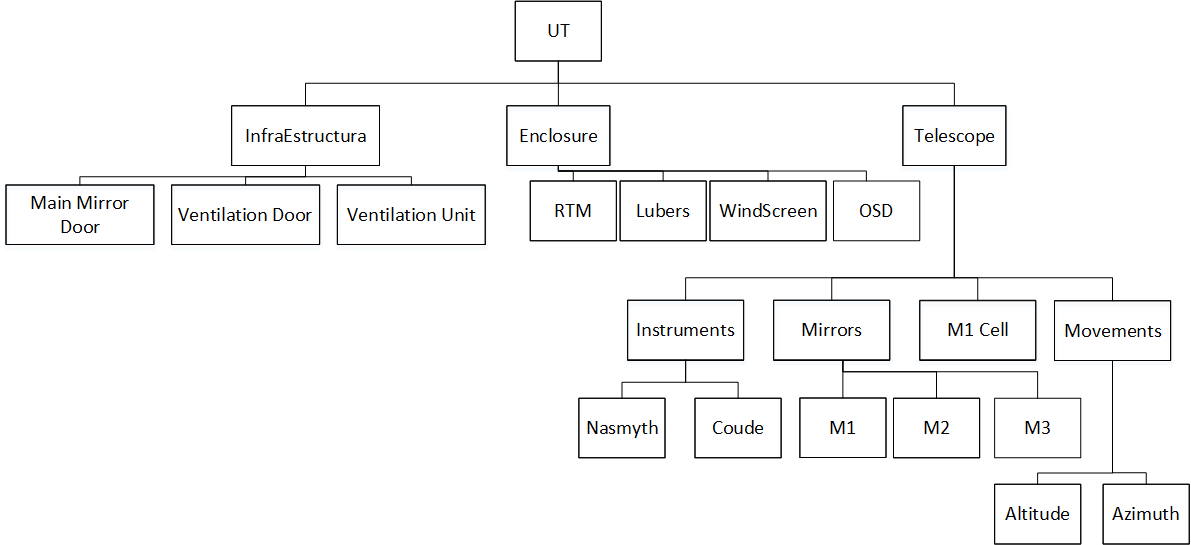
\includegraphics[width=\textwidth]{utorganigrama}
	    		\caption{Organigrama principal de un \textit{Unit Telescope}}
	    		\label{fig:UTorganigrama}
	    	\end{figure}    	
	    	\textit{Enclosure} (figura \ref{fig:UTexteriorpartes}): Es la estructura que se encarga de proteger el interior del telescopio de diferentes fuentes como la temperatura, polvo, rayos del sol. Como el telescopio necesita girar durante las noches de observación, el enclosure debe girar en sintonía con Azimut (giro de Base) además de tener ventanas que en la noche se abren para permitir la observación (Observation Slip Doors, OSD). El giro de este mismo se realiza gracias a los Rotation Mechanism (RTM) los cuales son dispositivos mecánicos en base a dos ruedas dispuestas en forma de balancín que son colocados a lo largo de toda la periferia (8 en total por telescopio) los que soportan el peso del Enclosure y gracias al contacto entre las ruedas y pista del Enclosure, al accionar sus motores permiten el giro del domo. \\
	    	Los luber y windscreens también juegan un rol fundamental en la protección del telescopio al momento de observar puesto que es usual tener grandes velocidades de viento, si estos pasaran directamente al telescopio podrían llegar a dañar los instrumentos o espejos dentro del telescopio, la manera de proteger el interior de los UT es mediante configuraciones que convierten la turbulencia del viento en un flujo laminar. Finalmente las OSD son las puertas principales que al abrirse dan paso al telescopio a recibir la luz del espacio.\\
	    	\begin{figure}[H]
	    		\centering
	    		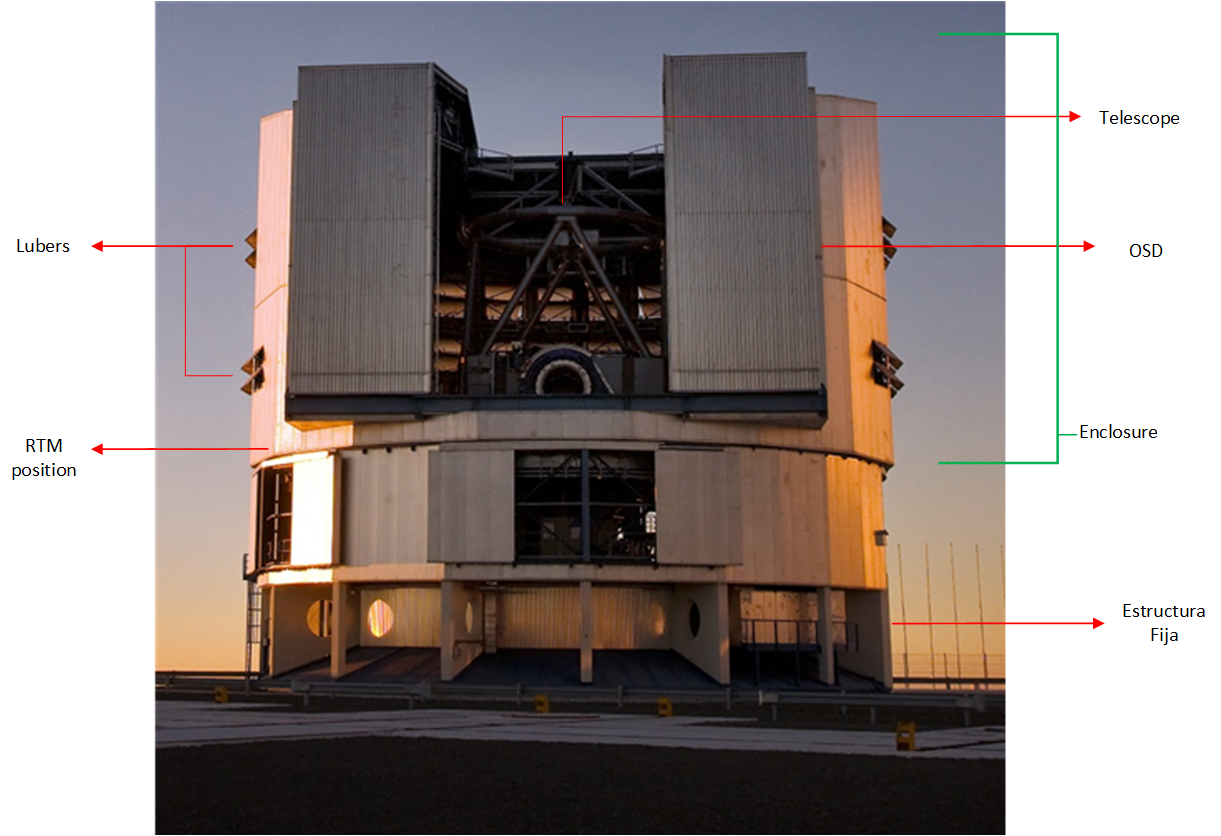
\includegraphics[width=\textwidth]{utpartesexterior}
	    		\caption{Vista exterior de un UT y sus partes principales}
	    		\label{fig:UTexteriorpartes}
	    	\end{figure}
	    	
	    	\textit{Telescopio} (figura \ref{fig:telescopioiso}): El telescopio es el corazón de cada UT, pues son ellos los encargados tanto de recibir la luz como de también de procesarla. Cada telescopio cuenta con un espejo principal de 8.2 [m] de diámetro (M1) los cuales son los que reciben la luz del cielo, seguido del espejo M2 y finalmente el espejo M3 que gracias a su posición en angulo de $45^\circ$ cumple la función de guiar la luz a Nasmyth A ó B, lugar donde se encuentran situado los instrumentos, también tiene una posición para dejar pasar la luz directamente hacia Coude. Una de las particularidades de el espejo principal es la de poseer óptica Activa (tecnología creada por la ESO) que permite corregir las deformaciones sufridas por el espejo percibidas al movimiento de altitud y azimut Esto se realiza mediante 150 soportes dispuestos en la parte baja del telescopio, que mediante software de control, logran percibir cambios en la forma del espejo y corregirlas rápidamente, la estructura que soporta este sistema es el llamado M1 cell estructura de acero de aproximadamente 10 toneladas, sus funciones son:
	    	\begin{figure}[H]
				\centering
				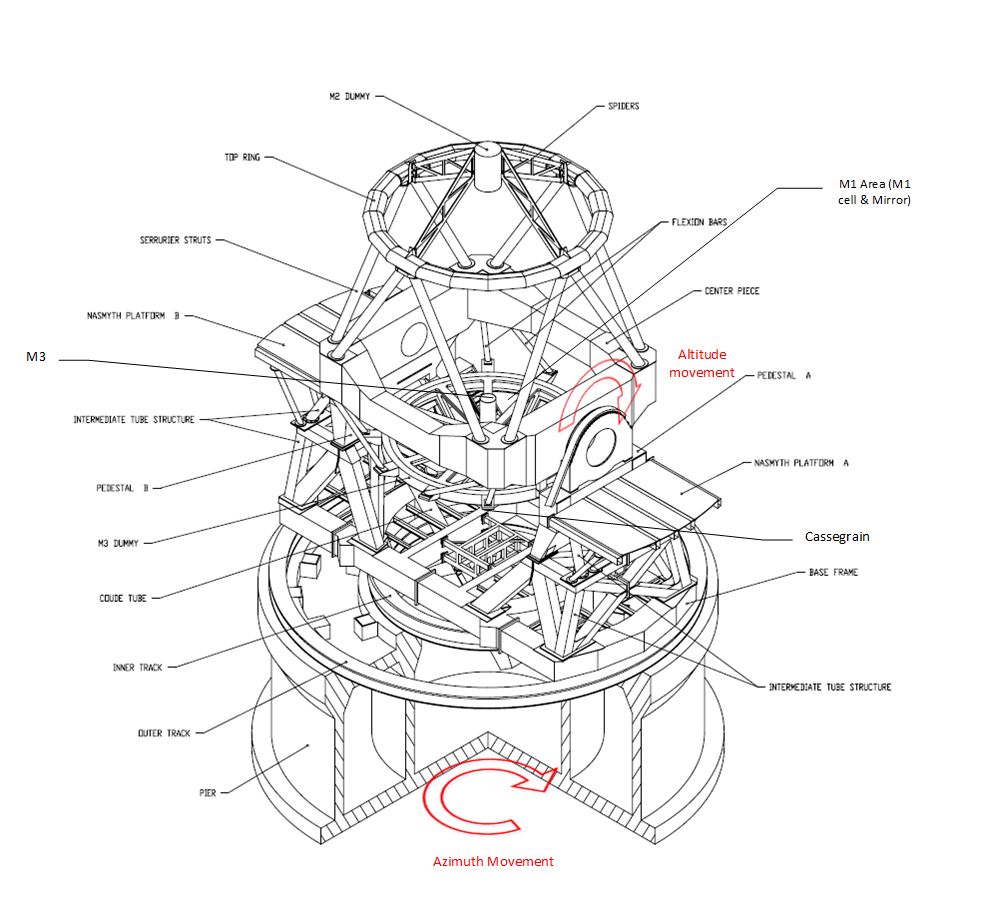
\includegraphics[width=\textwidth]{telescopioiso}
				\caption{Vista Isometrica del telescopio y sus componentes}
				\label{fig:telescopioiso}
			\end{figure}
			    	
	    	\begin{enumerate}
	    		\item Soportar el espejo de manera axial y lateral
	    		\begin{enumerate}
	    			\item Aplicar desde los 150 actuadores fuerzas axiales para deformar activamente el espejo.
	    			\item Proveer de promedios para ajustar remotamente la posición del espejo primario
	    		\end{enumerate}
    			\item Soportar el espejo terciario y seleccionar su posición para la selección del foco
    			\item Enfriar activamente el espejo primario	    		
	    	\end{enumerate}
	    	
    \section{Análisis del problema}
        \subsection{Antecedentes}
            El observatorio VLT (Cerro Paranal) está compuesto por cuatro telescopios de iguales características, conocidos como UT (unit telescope). Los equipos responsable del giro del domo, o enclosure (ver figura \ref{fig:UTexteriorpartes}), llamados RTM (Rotation Mechanism), serán el objeto de estudio y análisis del presente trabajo de título.
            
            El conjunto de telescopios en Paranal logró diez y seis años de operación ininterrumpida, teniendo el año 2013 un primer evento crítico sobre los RTM el cual hace suponer que la vida útil de estos sistemas está llegando a su termino. Con posterioridad, el año 2015, ocurre un segundo incidente que involucra un RTM; En esta ocasión un rodamiento falló, dejando por una semana uno de los telescopios fuera de operación. A partir de la información recopilada en el observatorio se realizó una tabla \ref{tab:RTMhistorial} que da cuenta de todas las intervenciones realizado hasta ahora de los mecanismos.
            \begin{table}[H]
                \centering
                \caption{Tabla con historial de modificaciones sobre RTM}
                \label{tab:RTMhistorial}
                \begin{tabular}{|l|l|p{7cm}|}
                \hline
                Fecha                            & Lugar     & Trabajo realizado                                      \\ \hline \hline
                Agosto 2013                      & UT1-RTM07 & Cambio de Boggie                                       \\ \hline
                \multirow{2}{*}{Septiembre 2014} & UT3-RTM08 & Se retiran ambos bogies, instalando desde UT3 a UT4    \\ \cline{2-3} 
                                                 & UT4-RTM08 & y modificando UT4 para finalmente ser instalado en UT3 \\ \hline
                Septiembre 2015                  & UT4-RTM05 & Cambio en rodamientos                                  \\ \hline
                Agosto 2016                      & UT1-RTM04 & Cambio de bogie (se instala uno nuevo)                 \\ \hline
                \end{tabular}
            \end{table}
             En el sistema de organización de trabajos de Paranal, existe una plataforma llamada PPRS  (Sistema de reporte de problemas) en la cual se recopilan las fallas mecánicas, electrónicas, eléctricas, de instrumentación, de software y de ciencias \& operaciones ocurridas en cada uno de los telescopios operativos en el año 2015. La \ref{tab:PPRStimes} resume los datos obtenidos tomando como referencia un solo telescopio (UT1) y los tiempos de las tareas asignadas para cada equipo de MSE. 
            \begin{table}[H]
                \centering
                \caption{Horas de trabajo por Equipo (PPRS)}
                \label{tab:PPRStimes}
                \begin{tabular}{|l|l|l|}
                \hline
                \multicolumn{3}{|c|}{Tareas y horas de trabajo asignadas por grupos en UT1}       \\ \hline \hline
                Grupo de Trabajo       & Cantidad de ordenes      & Carga de horas de trabajo   \\ \hline
                Mecánicos              & \textcolor{red}{347}   &\textcolor{red}{512.20} \\ \hline
                Software               & 180                      & 319.89                      \\ \hline
                Eléctrico/Electrónicos & 272                      & 178                         \\ \hline
                Otros                  & 38                       & 11.87                       \\ \hline
                Instrumentación        & 8                        & 10                          \\ \hline
                Total                  & 845                      & 1032.48 \\ \hline                   
                \end{tabular}
            \end{table}
            
            Se puede observar que cerca de un $50\%$ de los trabajos realizados corresponden a fallas mecánicas. Este $50\%$ se desglosa en los subsistemas a cargo del grupo Mecánico. En la tabla \ref{tab:PPRSmec} se detallan estos sistemas junto con el tiempo destinado a la reparación de cada falla.
            \begin{table}[H]
                \centering
                \caption{Horas perdidas de observación y horas usadas en la reparación de los sistemas mecánicos.}
                \label{tab:PPRSmec}
                \begin{tabular}{|l|c|p{4cm}|p{4cm}|}
                \hline
                \multicolumn{4}{|c|}{Cantidad de horas perdidas por problemas reportados}                                                              \\ \hline \hline
                \multicolumn{1}{|c|}{Sistema} & Cantidad de tareas & Horas perdidas de observación & Horas (totales) usadas en reparación del problema \\ \hline 
                RTM                           & \textcolor{red}{24}& \textcolor{red}{71.63}        & \textcolor{red}{235.60}  \\ \hline
                Windscreen                    & 26                 & 4.78                          & 66.57                                             \\ \hline
                OSD                           & 65                 & 4.18                          & 65.55                                             \\ \hline
                Thermal                       & 132                & 1.60                          & 56.50                                             \\ \hline
                Louvers                       & 19                 & 1.18                          & 27.47                                             \\ \hline
                Seal                          & 22                 & 0.83                          & 23.36                                             \\ \hline
                MMD                           & 2                  & 0.75                          & 17.15                                             \\ \hline
                Otros                         & 30                 & 0.65                          & 10.50                                             \\ \hline
                VDS                           & 17                 & 0.33                          & 6.50                                              \\ \hline
                Park Enc                      & 10                 & 0.17                          & 4                                                 \\ \hline
                TOTAL                         & 347                & 86.10                         & 512.20                                            \\ \hline
                \end{tabular}
            \end{table}            
            Como se observa en la tabla \ref{tab:PPRSmec}, la mayor cantidad  de horas hombres del grupo mecanico se destinó a arreglar fallas en RTM ($46\%$ del total) esto supuso un $78.91 \%$  de tiempo perdido para observaciones astronómicas, actividad fundamental de todo observatorio.
            
            Estos resultados nos permiten concluir  que los Rotation Mechanism pueden ser considerados un sistema crítico entre los del equipo de mecánica. Estas fallas impactan la actividad fundamental de la empresa (tanto a nivel de observaciones como de mantención) por lo que el grupo de mecánica esta en busca de sistemas para aumentar la confiabilidad de los RTM o de caracterizar en el estado que se encuentran, una de las posibles técnicas de monitoreo escogido a analizar son las vibraciones mecánicas.
            
            Debido a que estos equipos se componen de elementos mecánicos en rotación, esta memoria tiene como finalidad estudiar la factibilidad técnica del uso de análisis de vibraciones en los RTM con el objetivo de encontrar anomalías su funcionamiento. El desafió de trabajar en estos equipos es la alta carga y baja velocidad a la que se encuentra en su operación normal haciendo difícil el análisis de vibraciones ya que no se generan fuerzas dinámicas de gran amplitud. Estos equipos no llegan a superar las 15 Revoluciones por minuto en su capacidad máxima de giro. Por esta razón, se estudiarán dos técnicas de análisis para equipos que cumplen con estas condiciones de operación: Promedios en frecuencia y aplicación de la correlación de curtosis mediante curtogramas. A través de ambas técnicas se verá la factibilidad de encontrar fallas en los rodamientos de los RTM. 
    \Section{Objetivos}
        \subsection{Objetivo General} \label{ssec:objgral}
            Estudiar la factibilidad de implementar un método de análisis de falla mediante vibraciones mecánicas que permitan caracterizar el estado de equipos que trabajan a baja velocidad y con alta carga.
            \subsection{Objetivo Específico}
            \begin{itemize}
                \item Analizar técnicas de análisis de señal aplicables a equipos con las características mencionadas en \ref{ssec:objgral}.
                \item Crear una pauta de medición que permita estandarizar las señales de vibraciones de los RTM
                \item Programar un modelo computacional que permita analizar las mediciones realizadas.
                \item Presentar análisis y resultados            
            \end{itemize} 
    		\newpage
    \section{Medición de la vibración}
        \subsection{Etapas de la medición}
	        Las etapas a seguir para la medición y análisis de las vibraciones se clasifican en las siguientes partes:
			\begin{enumerate}
				\item \textbf{\textit{Transductora}}: Etapa donde el sensor de vibraciones transforma la señal análoga (vibración del equipo) en una señal eléctrica \textbf{proporcional} a la magnitud medida.
					
				\item \textbf{\textit{Acondicionamiento de la señal eléctrica}}: Algunas señales entregadas por el sensor no pueden ser registradas o introducidas directamente, es decir, necesitan ser acondicionadas previamente. Por ejemplo, la señal de un sensor de vibración necesita de una amplificación de la señal en orden de ser percibida. Por lo general los sensores de aceleración (acelerómetros piezoeléctricos) usados en la industria vienen con un preamplificador (ICP, integrated circuit piezoelectric) de la señal integrado, haciendo que esta etapa no sea percibida.
					
				\item \textbf{\textit{Procesamiento  y medición}}: Etapa fundamental del análisis de vibración, pues esta etapa consiste en usar técnicas o procedimientos para sacar la mayor información de la información, el procesamiento clásico de la medición de vibraciones es el análisis de frecuencia mediante el uso de la transformada de Fourier. Otro ejemplo de procesamiento y medición es capturar los valores RMS, valor pico, valor pico-pico.
					
				\item \textbf{\textit{Registro}}: Consiste en guardar (registrar) los datos medidos y procesados, este puede ser directamente en el equipo transductor como en un Computador.
			\end{enumerate} 
			Existen diferentes tipos de sensores de vibraciones típicos, dentro de los cuales los de uso más común son
			\begin{enumerate}
				\item Desplazamiento relativo sin contacto
				\item Desplazamiento relativo sin contacto
				\item Sensor de velocidad o velocímetro
				\item Sensor de aceleración o acelerómetro.
			\end{enumerate}
			Para efectos de medición, se utilizará un sensor de aceleración (\ref{fig:acellpartes}) piezoeléctrico, el cual es el tipo de sensor usado en mayoría. El principio de funcionamiento son los materiales piezoeléctricos (como el cuarzo) que tienen la propiedad de que al aplicarles una fuerza externa en dirección de su polarización se genera una carga eléctrica entre sus superficies, la cual es proporcional a la fuerza aplicada y por ende, a su aceleración. \\			
			\begin{figure}[t]
				\centering
				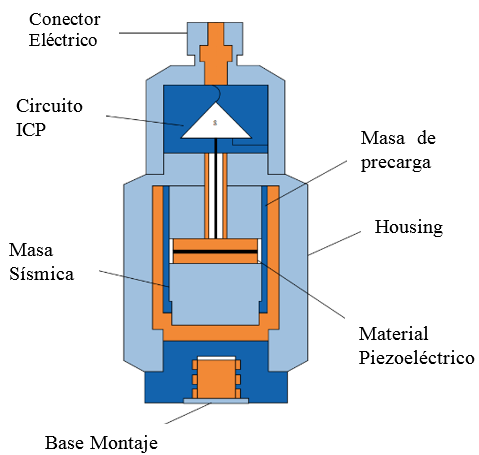
\includegraphics[width=0.5\textwidth]{partesacelerometro}
				\caption{Esquema de un acelerómetro y sus partes principales}
				\label{fig:acellpartes}
			\end{figure}
		\subsection{Transformada discreta de Fourier}
			La transformada de Fourier tiene un trasfondo puramente matemático, y es aplicable solo a funciones continuas, Es por esto que se introduce el concepto de Transformada Discreta de Fourier, computada mediante el algoritmo FFT (ingles \textit{Fast Fourier Transform}).
			
			\begin{equation}
				X\left[k\right]=\ \sum_{n=0}^{N-1}x[n]e^{-\frac{2\pi{}i}{N}kn}
				\label{eq:discretafourier}
			\end{equation}
			
			Uno de los grandes limitantes es la gran cantidad de operaciones que deben hacerse para su cálculo, específicamente $ O( n^2 ) $. Mediante manipulación matemática, en el año 1965, James Cooley y John Tukey publicaron una manera general de un algoritmo capaz de reducir el número de operaciones a $O(n log(n)$ (figura \ref{fig:diffftdft}), existen numerosos algoritmos computacionales para el cálculo de la FFT, uno de los más famosos y gratuitos es el FTTW (Fastest Fourier Transform of the West).
			\begin{figure}
				\centering
				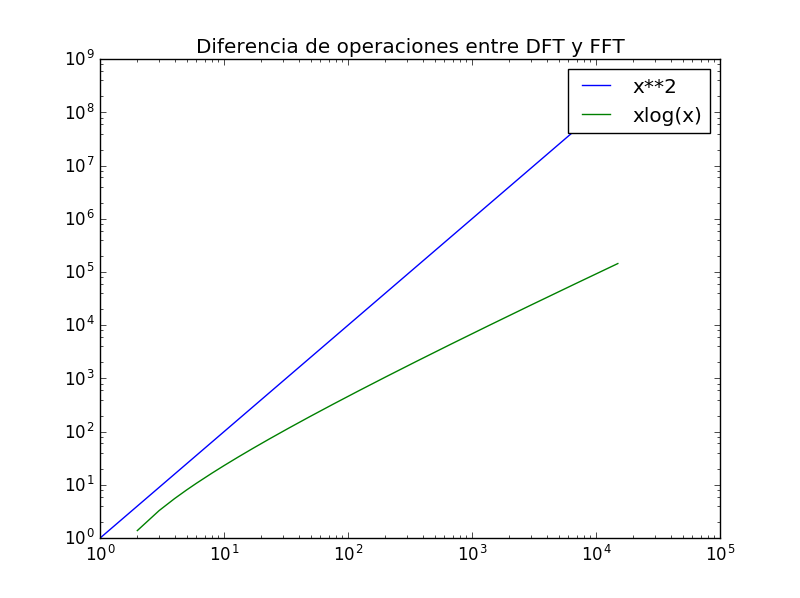
\includegraphics[width=0.5\textwidth]{DiferenciaentreDFTyFFT}
				\caption{Diferencia en operaciones entre FFT y DFT}
				\label{fig:diffftdft}
			\end{figure}
    	\subsection{Densidad Espectral}
	 		La densidad espectral de una señal nos da cuenta de como esta distribuida la potencia o la energía de dicha señal en cada frecuencia de la cual está formada. Para procesos transcientes en el tiempo (aquellos que empiezan y terminan en cero en amplitud) es posible usar densidad espectral con relación a su energía (ejemplo, prueba de impacto). En el caso de señales continuas y estacionarias donde la cantidad de energía medida es proporcional al tiempo de observación, deben ser medidas en unidades de potencia, es decir, de energía por unidad de tiempo.\\
	 		Básicamente la PSD (\textbf{Power} Spectrum Density) se calcula como el valor esperado de la transformada de Fourier con la señal al cuadrado (potencia) (ecuación \ref{eq:psd})
	 		\begin{equation}
		 		S_{xx}(\omega) = \lim_{T\to\infty}(\textbf{E}\lvert \hat{x}_T(\omega)\rvert^2)
		 		\label{eq:psd}
	 		\end{equation}
	 		donde $S_{xx}(\omega)$ es el valor de la PSD.
	 		Uno de los métodos para aproximar la PSD es el algoritmo propuesto por P.D Welch \cite{Welch1967}, el cual propone calcular la PSD a través de la Transformada de fourier en segmentos de la señal original (periodogramas) para luego promediar cada uno de ellos. Cada segmento de la señal original es multiplicada por una función ventana. Los parámetros para el calculo de la PSD mediante el método de Welch son:
	 		\begin{itemize}
	 			\item \textbf{x}: Arreglo con los datos de la serie de tiempo
	 			\item \boldmath{$f_s$}: frecuencia de sampleo de la serie de tiempo
	 			\item \textbf{window}: Ventana a aplicar sobre x
	 			\item \textbf{nperseg}: Número de puntos de la serie de tiempo por segmento
	 			\item \textbf{noverlap}: Número de puntos a superponer entre segmentos
 			\end{itemize}
	 		Los cuales devuelven dos series de datos:
	 		\begin{itemize}
	 			\item \textbf{f}: arreglo con las frecuencias de sampleo.
	 			\item \boldmath{$P_{xx}$}: PSD del arreglo x.
	 		\end{itemize}
  		\subsection{Detección de fallas en rodamientos}
 			El rodamiento es un elemento mecánico utilizado en casi la mayoría de los equipos rotatorios, es por eso que es de vital importancia el análisis o monitoreo de estos componentes en el mantenimiento predictivo.
 			
 			Dentro del ciclo de operación de un rodamiento, aunque este sea montado de manera correcta, con una correcta lubricación, manteniéndolo libre de elementos contaminantes (agentes externos) y calculándolo para una correcta operación se puede decir que el rodamiento estará libre de fallas exceptuando una: la falla por fatiga, la cual no puede ser evitada debido a su tiempo de operación o vida útil. Es por esto que la evolución de la falla de un rodamiento a través del tiempo se puede clasificar en cuatro etapas y es esta clasificación por la cual, la experiencia dice que este tipo de falla ocurre en aproximadamente el $80\%$ de las veces
 			\begin{itemize}
 				\item Etapa 1: El primer indicio de falla en un rodamiento es una grieta a nivel microscópico y sub-superficial, generalmente localizado en el punto de mayor carga del rodamiento (punto de contacto entre el elemento rodante y la pista externa), en esta etapa la detección de la grieta (a nivel microscópico) es imposible de detectar mediante el uso de un acelerómetro y espectros frecuentes, por lo que se deben emplear técnicas mas complejas siendo una de ellas llamada IDF (Incipient Detection Failure) la cual aprovecha la frecuencia natural del acelerómetro para amplificar esta señal de baja amplitud 
 				\item Etapa 2: Una vez que se genero la grieta sub-superficial, esta comenzará a propagarse hacia la superficie produciéndose una pequeña fisura o picadura en el elemento. Esta falla es apenas visible para el ojo humano. Al existir esta picadura, en el momento en el que una bola pasa por esta, se produce un efecto mazo-campana que hace que la bola existe las frecuencias naturales de la pista siendo estas frecuencias de alta frecuencia pero de baja amplitud
 				\item Etapa 3: El paso de las bolas sobre la picadura hace que la picadura aumente en tamaño, haciendo que las componentes de frecuencias en el espectro de velocidad en los elementos del rodamiento (frecuencias cuales son propias de cada elemento del rodamiento -pista externa, interna, jaula o bolas- dependiendo de donde se localiza la picadura [tabla \ref{tab:frecuenciasrodamiento}]) 
 				\item Etapa 4: La falla catastrófica es inminente debido a que la falla ya es de gran magnitud dentro del rodamiento, es de esperar también que el daño ya sea múltiple en los elementos lo que hace que aparezcan mas componentes de falla de los elementos del rodamiento en el espectro y el daño en pistas puede estar distribuida a su largo y no solo concentrado en un punto.
 			\end{itemize}
 			Como se menciono dentro de las etapas de falla de un rodamiento, los impactos generados a partir de un defecto en alguno de los elementos del rodamiento producen una excitación (vibración) cada vez que un elemento rodante hace contacto con la superficie dañada. Esta excitación de los elementos suele ser periódica con relación directa con la velocidad de los elementos rodantes y la geometría del rodamiento.
 			
 			\begin{center}
 				\begin{table}
 					\caption{nomenclatura de las frecuencias características de rodamiento}
 					\label{tab:frecuenciasrodamiento}
 					\begin{tabular}{| >{\centering\arraybackslash}m{0.4\linewidth} | >{\centering\arraybackslash}m{0.1\linewidth} |>{\centering\arraybackslash}m{0.4\linewidth}| } 		
 						\hline
 						Frecuencia característica & \scriptsize{Acrónimo} & Fórmula \\ \hline \hline
 						Frecuencia de paso de los elementos rodantes sobre la pista externa.
 						(Ball pass frequency of outer race) & BPFO & $$\frac{RPM\cdot n}{2}\cdot \left (1-\frac{d\cdot\cos{\theta}}{d_{m}}\right )$$ \\ \hline
 						Frecuencia de paso de los elementos rodantes sobre la pista interna.
 						(Ball pass frequency of inner race) & BPFI & $$\frac{RPM\cdot n}{2}\cdot\left (1+\frac{d\cdot\cos{\theta}}{d_{m}}\right )$$ \\ \hline
 						Frecuencia de rotación de la jaula contenedora de las bolas (Fundamental train frequency) & FTF & $$\frac{RPM}{2}\cdot \left (1+\frac{d\cdot\cos{\theta}}{d_{m}}\right )$$ \\ \hline
 						Frecuencia de giro de los elementos rodantes & BSF & $$\frac{RPM \cdot  d_{m}}{2d}\left[1-\left(\frac{d}{d_{m}}\right)^2 \cos^2(\theta)\right]$$ \\ \hline
 					\end{tabular}
 				\end{table}					
 			\end{center}
 		    \begin{figure}
 			    \centering
 			    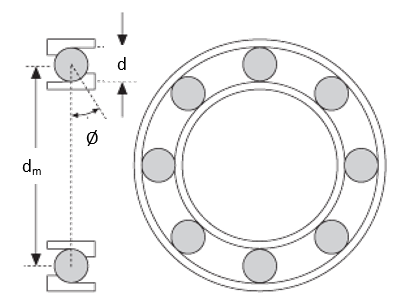
\includegraphics[width=0.6\linewidth]{rodamientoindices}
			    \caption{nomenclatura usada en tabla \ref{tab:frecuenciasrodamiento}}
 			    \label{fig:rodamientopartes}
 		    \end{figure}
 		    Donde:
     		\begin{itemize}
     			\item $n$: número de elementos rodantes
     			\item $d$: diámetro de los elementos rodantes
     			\item $d_{m}$: diámetro entre los centros de los elementos rodantes
     			\item $RPM$: revoluciones por minuto de giro del rodamiento
     		\end{itemize}
            La señal que se obtiene al medir un rodamiento poseen un comportamiento especial dependiendo del elemento que presente la falla, en especial aquellos rodantes (pista interna -En la mayoría de las aplicaciones en la cual gira-,elementos rodantes), pues estos están constantemente pasando y saliendo por la zona de alta carga, originándose una señal modulada en amplitud, pues el elemento al chocar en la zona de alta carga tendrá una respuesta mayor en amplitud que cuando esta misma pase por la zona de mínima carga.
         	\begin{figure}
        		\centering
        		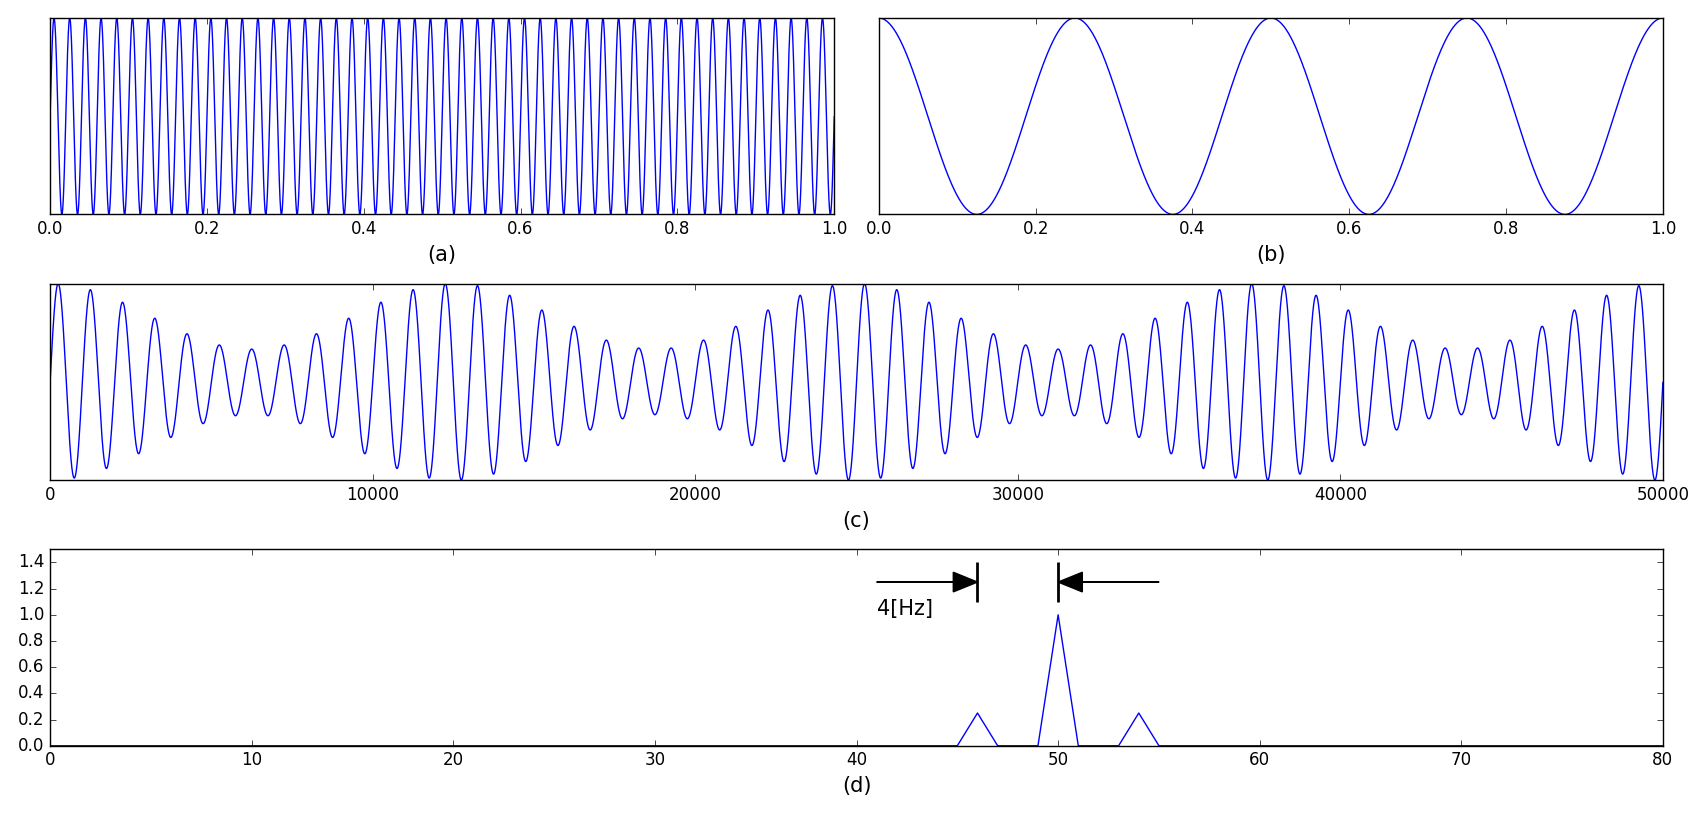
\includegraphics[width=\linewidth]{modulacion}
        		\caption{Ejemplo de señal modulada en amplitud}
        		\label{fig:modulacion}
        	\end{figure}
	
		    \subsubsection{Señales moduladas en amplitud}
    			La modulación en amplitud consiste en una interacción particular entre dos señales diferentes, donde la amplitud de una señal varía en relación a la señal transmitida o la señal modulada, es decir, donde por lo general la frecuencia de la onda portadora es mayor a la onda modulada, matemáticamente se tiene la siguiente relación para la modulación en amplitud: 
    			
    			Una señal portadora de forma trigonométrica:\\
    			
    			\begin{equation}
    				p(t) = A \cdot \sin \left(2 \pi f_{p}t \right)			
    			\end{equation}
    			
    			Una señal la cual sera modulada por la señal portadora: 
    			
    			\begin{equation}
    				m(t)= M \cdot \sin \left(2 \pi f_{m} t \right) 
    			\end{equation}
    			
    			Finalmente, la modulación con la señal portadora se expresa como: 
    			
    			\begin{equation}
    				y(t)=\left[m(t)+1\right ]\cdot p(t)				
    			\end{equation}
    			donde: 
    			
    			\begin{itemize}
    				\item $p(t)$: Onda portadora
    				\item $m(t)$: Onda a montar
    				\item $A$ y $M$: Amplitud de cada onda
    				\item $f_{p}$ y $f_{m}$: Frecuencia de cada onda
    				\item $y(t)$: señal modulada en amplitud
    			\end{itemize}
    			
    			Un ejemplo de modulación en amplitud se puede apreciar en la imagen \ref{fig:modulacion} donde se tienen dos señales, (a) con una frecuencia de $50[Hz]$ y (b) con una frecuencia correspondiente de $4[Hz]$, en (d) se puede ver la forma característica de la modulación en amplitud que consiste en una frecuencia central, correspondiente a la señal portadora y dos frecuencias a ambos lados correspondientes a la onda montada, la distancia entre estas frecuencias es equivalente a la de la onda montada. En la práctica las modulaciones en amplitud suelen contar con mayor numero de lineas laterales debido a los armónicos de la señal.\\
    			
    			Estas señales moduladas en fallas en rodamientos, la señal moduladora contiene la información acerca de las fallas características es que existen técnicas (procesamiento de la señal) para extraer las frecuencias de interés Una de estas herramientas es calcular hacer uso de la señal analítica (señal que se caracteriza por no contener frecuencias negativas) para así calcular la envolvente de la señal usando la transformada de Hilbert, la cual se define, para una señal arbitraria $f(t)$ como \cite{Boashash1992}:
    			\begin{equation}
    				H \{f(t)\} = p.v \cdot \int_{-\infty}^{\infty} \frac{f(t-\tau)}{\pi \tau} d\tau
    			\end{equation}
    			donde $p.v$ corresponde al valor inicial de Cauchy. Una señal con valores reales, como las medidas en vibraciones puede ser representada de forma analítica de la siguiente manera:\\
    			\begin{equation}
    				s_{a}=s(t)+j \cdot H[s(t)]
    			\end{equation}
    			de esta manera, analíticamente, la señal esta representada de manera compleja, por lo que puede expresarse de manera compleja de la forma:\\
    			\begin{equation}
    				s_{a}(t) = s_{m}(t) \cdot e^{j\phi (t)}			
    			\end{equation}
    			donde $|s_{a}|$ corresponde a la amplitud instantánea y $\arg\left (|s_{a}(t)|\right )=\phi(t)$ a la fase. Dos ejemplos de envolventes mediante la transformada de Hilbert pueden verse en la imagen \ref{fig:hilbert1} y \ref{fig:hilbert2}
    			\begin{figure}[H]
    				\centering
    				\begin{subfigure}[b]{\linewidth}
    					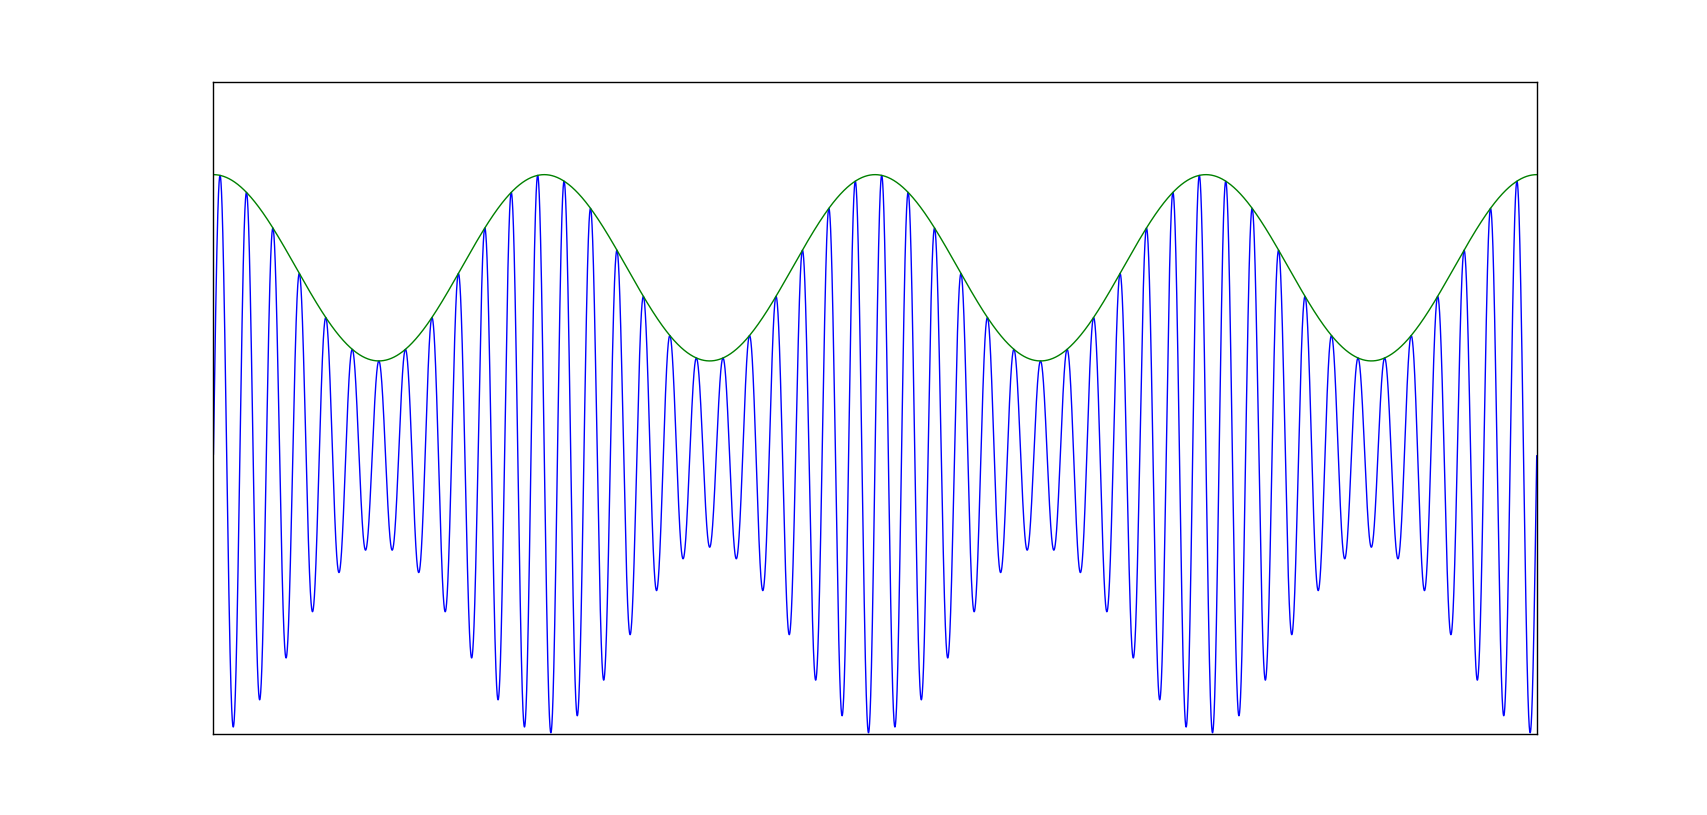
\includegraphics[width=0.9\linewidth]{hilbert1}
    					\caption{Envolvente de señal pura}
    					\label{fig:hilbert1}
    				\end{subfigure}
    				\begin{subfigure}[b]{\linewidth}
    					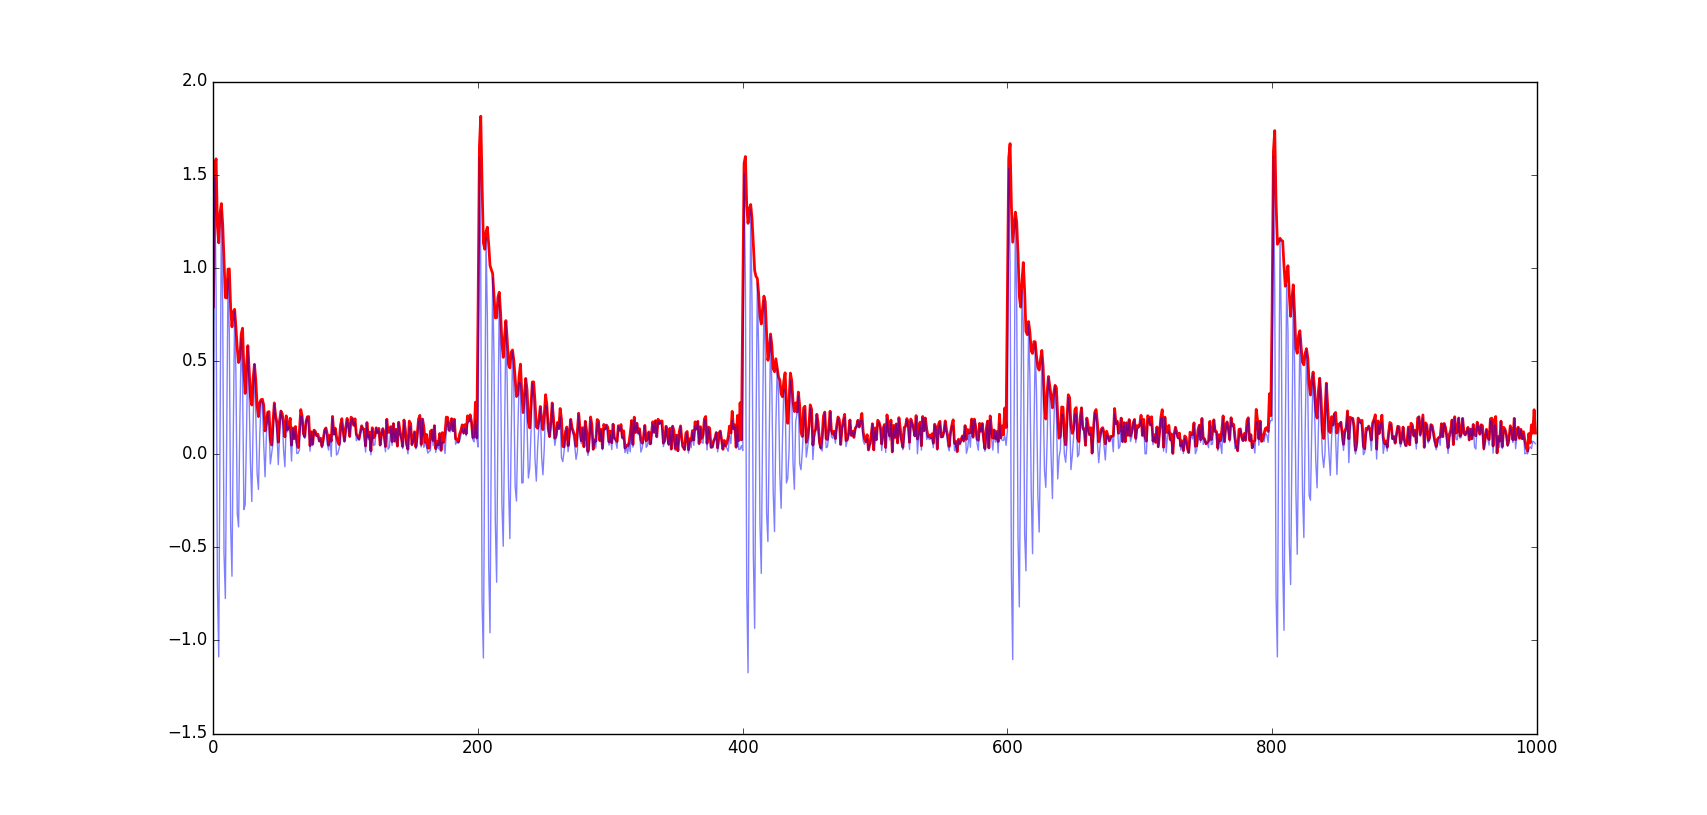
\includegraphics[width=0.9\linewidth]{hilbert2}
    					\caption{Envolvente de una señal impulsiva con ruido gaussiano}
    					\label{fig:hilbert2}
    				\end{subfigure}
    				\caption{Ejemplos de envolvente mediante transformación de Hilbert}
    				\label{fig:hilbert}						
    			\end{figure}
    		El procedimiento para aislar la señal de interés consiste en los siguientes pasos:
    		\begin{enumerate}
    			\item {Calcular FFT de la señal a analizar}
    			\item Seleccionar filtro pasa banda procurando dejar la zona donde se ve comportamiento de modulación en amplitud
    			\item En el caso de querer estudiar severidad, debe aplicarse una ganancia a la señal filtrada
    			\item Calcular la señal analítica de la señal mediante la transformada de Hilbert para calcular envolvente
    			\item Calcular FFT de la señal envolvente
    			\item Corroborar si aparecen tonos de rodamientos (BPFO,BPFI...) 
    		\end{enumerate}
		
	\section{Análisis en equipos a baja velocidad}
		\subsection{Desafío a bajas revoluciones}
		    Predecir la presencia de fallas en equipos que operan a bajas revoluciones utilizando las técnicas de espectros resulta ser una tarea difícil de llevar a cabo, principalmente debido a que el giro de estos equipos por lo general no son lo suficientemente rápidos como para generar las fuerzas dinámicas significantes como para manifestarse en la forma de onda del fenómeno que se esta midiendo por lo que esta señal, en caso de no ser nula, resulta ser de baja amplitud pasando estas desapercibidas por el nivel de ruido del entorno. Las máquinas consideradas de bajas revoluciones son aquellas que giran entre 6 y 300 ciclos por minuto \cite{robinsonjc}			
		\subsection{Estado actual de técnicas a bajas revoluciones}
		    Debido a que en este tipo de máquinas las fuerzas dinámicas suelen ser bajas es que las manifestaciones clásicas de fallas suelen no aparecer exceptuando fallas localizadas como lo son por ejemplo fallas en rodamientos que generan señales con características no estacionarias y transcientes (Señales que empiezan y terminan en cero en un tiempo finito \cite{dlinonstationary}). A continuación se resumen tres técnicas usadas en el análisis a baja velocidad que tienen como objetivo el análisis de fallas en rodamientos:
			\subsubsection{Análisis de forma de Onda}
		        Como el efecto o falla de rodamiento es de tipo localizado, cada vez que un elemento rodante pasa por la falla, se produce un impacto que produce una vibración no estacionaria. El análisis de la forma de onda de aceleración permite identificar los impactos producidos por el paso de los elementos rodantes. Un ejemplo de este análisis esta propuesto en \textit{análisis de vibraciones aplicados a las maquinas rotatorias de baja velocidad} \cite{pedrosaav}
		        \begin{figure}
		            \centering
		            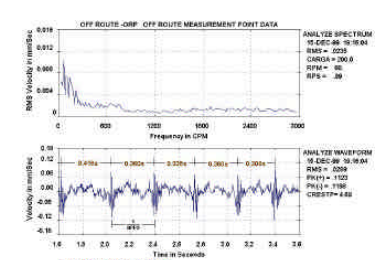
\includegraphics{formaondasaavedra}
		            \caption{Espectro y forma de onda de rodamiento con pista externa defectuosa y velocidad variable}
		            \label{fig:rodsaav}
		        \end{figure}
		        En la figura \ref{fig:rodsaav} se muestra tanto la forma de onda como el espectro de frecuencia medido en un agitador que presenta fallas en la pista externa del rodamiento, la velocidad nominal del equipo son 60 rpm. Si se analiza el espectro tomado, no se puede observar la componente de frecuencia correspondiente al rodamiento. Sin embargo, si se analiza la serie de tiempo, se pueden notar impactos a un tiempo aproximadamente el inverso del tono de rodamiento BPFO confirmando una existencia de falla en rodamiento
			     \subsubsection{Análisis Espectral promediando en frecuencia}
			        Esta técnica se basa en promediar diferentes mediciones realizadas de igual manera con el fin de promediar los espectros, obviando así la diferencia de fase que se pueda presentar entre mediciones. Esto hace que tanto el ruido electrónico como señales del entorno (aleatorias) disminuyan manteniendo en alto aquellas que no varían de manera aleatoria (señal de interés) esto mejora la relación señal/ruido de las mediciones. Un factor importante es que para esta técnica también se necesita una alta resolución en frecuencia (numero de lineas). Esto aumentando el tiempo de adquisición de la señal a analizar.
			        En la figura \ref{fig:fftpromedio} puede verse como mejora el espectro al aumentar el numero de promedios y el numero de lineas (Fuente: \cite{pedrosaav}).
        			\begin{figure}[H]
        				\centering
        				\begin{subfigure}[b]{\linewidth}
        				    \centering
        					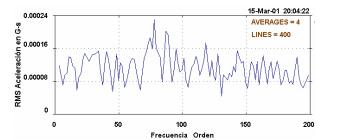
\includegraphics{fftpromedio1}
        					\caption{Espectro con 4 promedios y 400 líneas de resolución}
        					\label{fig:fftpromedio1}
        				\end{subfigure}
        				\begin{subfigure}[b]{\linewidth}
        				    \centering
        					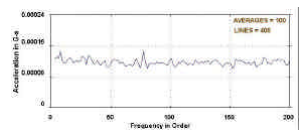
\includegraphics{fftpromedio2}
        					\caption{Espectro con 100 promedios y 400 lineas de resolución}
        					\label{fig:fftpromedio2}
        				\end{subfigure}
        				\begin{subfigure}[b]{\linewidth}
        				    \centering
        					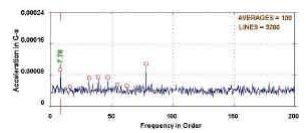
\includegraphics{fftpromedio3}
        					\caption{Espectro con 100 promedios y 3200 lineas de resolución}
        					\label{fig:fftpromedio3}
        				\end{subfigure}
        				\caption{Ejemplo de espectros para diferente configuración de promedios y resolución}
        				\label{fig:fftpromedio}
        			\end{figure}	
        		\subsubsection{Curtosis correlacionada y curtogramas}
        		    Este último método es una herramienta estadística para analizar ondas no estacionarias (como rodamientos) debido a que es capaz de indicar la presencia de series transientes y las frecuencias locales en el dominio de frecuencias. La idea general es la de modelar la señal como una suma lineal entre una señal transiente (débil) y ruido, es decir:
        		    \begin{equation}  		         		        
        		        Y(t)=X(t)+N(t)
        		    \end{equation}
        		    en el cual X(t) es la señal transiente y N(t) es ruido. 
        		    
        		    Una manera de analizar este tipo de señal es considerando indicadores estadísticos sensibles a la señal con series de picos (abrupta). Un indicador útil es la curtosis la cual adopta valores altos cuando la señal es del tipo X(t) (figura \ref{fig:curtosiss}) y idealmente cero cuando se tiene sonido de fondo N(t).
        		    \begin{figure}
        		        \centering
        		        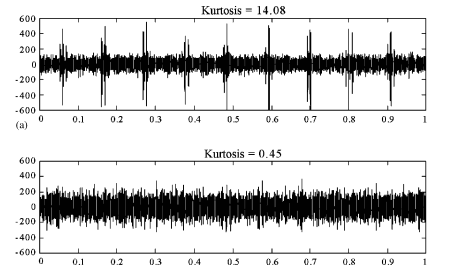
\includegraphics{kurtosis}
        		        \caption{curtosis para dos tipos de señales}
        		        \label{fig:curtosiss}
        		    \end{figure}
        		    La curtosis espectral (SK) presentada por Antoni propone la aplicación de la curtosis localmente para diferentes bandas de frecuencias, ayudando así a evitar que las vibraciones de señales fuertes, repartidas en un rango largo de frecuencias, intervengan con la señal de interés, este proceso de filtrado se le conoce como curtosis espectral la cual se calcula mediante \cite{antoni2006spectral}:
        		     \begin{equation}
        		        K_x(f)= \frac{\langle |H(n,f)|^4 \rangle}{\langle |H(n,f)|^2 \rangle^2}-2
        		    \end{equation}
        		    donde:
        		    \begin{equation}        		        
        		        \langle f(n) \rangle = \lim_{N\to\infty} \frac{1}{N} \sum_{N} f(n)
        		    \end{equation}
        		    y $|H(t,f)|$ representa la envolvente compleja de la señal x(t) a la frecuencia f.
        		    
        		    Las propiedades principales de la SK son:
        		    \begin{itemize}
        		        \item la SK the un proceso estacionario es una constante en función de la frecuencia
        		        \item la SK de un proceso Gaussiano Estacionario es 0
        		        \item en la presencia de ruido ($N(t)$), la SK del proceso no estacionario x(n) es:
        		    \end{itemize}
        		    \begin{equation}
        		        K_y(f)=\frac{K_x(f)}{\left[1+\rho(f)\right]^2}
        		    \end{equation}
        		    donde:
        		    \begin{enumerate}
        		        \item $K_x(f)$: SK de señal X(t)
        		        \item $K_y(f)$: SK de señal Y(t)
        		        \item $\rho(f)$: relación ruido-señal
        		    \end{enumerate}
        		    Esta fórmula indica que si la relación señal-ruido es alta, $K_x(f)$ tiende a ser igual a $K_y(f)$ y $K_y$ tiende a  0 cuando la relación es baja.  
        		    las propiedades (1) y (2) muestran la habilidad de la SK para detectar, caracterizar y localizar en frecuencia la parecencia de señales no estacionarias escondidas en los datos.
    			    
    			    SK se ve afectada por el largo de la ventana elegida. Es por eso que Antoni \cite{antoni2006spectral} propone el uso de la transformada de Fourier corta en tiempo para calcular SK con diferentes tamaños de ventana y poder seleccionar el ancho de banda en frecuencia donde la curtosis es mayor. Esta técnica introduce el concepto de curtogramas, el cual es una representación gráfica de SK para diferentes anchos de banda y centradas a diferentes frecuencias, herramienta que debido a su rápido calculo está siendo aplicado en el análisis de falla en rodamiento actualmente.
    			    \begin{figure}[H]
    			        \centering
    			        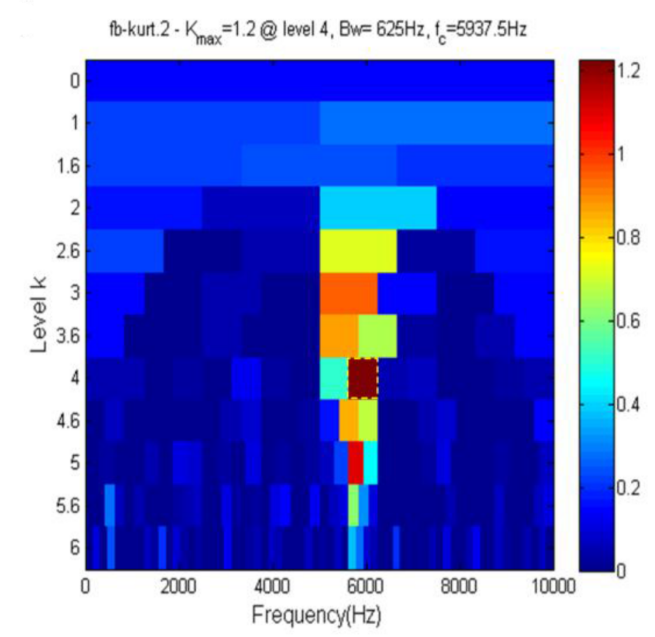
\includegraphics[width=0.5\linewidth]{ejemplokurtograma}
    			        \caption{Ejemplo curtograma}
    			        \label{fig:curtogramaejemplo}
    			    \end{figure}
    			En la figura \ref{fig:curtogramaejemplo} se observa un ejemplo de curtograma para una señal, se puede observar que el mayor valor de curtosis se encuentra en torno a los $6000[Hz]$ con un ancho de frecuencia de $\Delta f= 1250 [Hz] $, el cual se encuentra en el nivel $k=4$. Estos datos permiten la elección de un filtro para demodular el tipo de señal buscada, centrando el filtro en $f_c$ con un ancho de filtro de $\Delta f$.
    			Hoy en día existen varios trabajos relacionados con encontrar fallas en rodamientos empleando la técnica de los curtogramas, a continuación se presenta uno de ellos tomado de \cite{Konstantinos2016} en el cual se detectan fallas en rodamientos en un motor lubricante dentro de un barco.
    			
    			El proceso de análisis de la señal se muesta en la tabla \ref{fig:procesokurtograma}
    			\begin{figure}
    			    \centering
    			    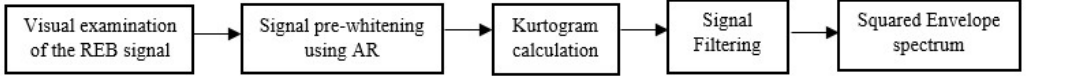
\includegraphics[width=0.7\linewidth]{procesokurtograma}
    			    \caption{Pasos para demodulacion de señal}
    			    \label{fig:procesokurtograma}
    			\end{figure}
    			
    			El autor del trabajo analiza la señal a una tasa de muestreo de $44.1 [kHz]$ sobre un rodamiento modelo 6222 SKF el cual presenta fallas en su pista externa, por lo que es de esperar componentes en el espectro correspondientes al tono de rodamiento BPFO (4.07X)
    			la serie de tiempo junto con el espectro se muestran en la figura \ref{fig:ejkurtograma}
    			\begin{figure}
    			    \centering
    			    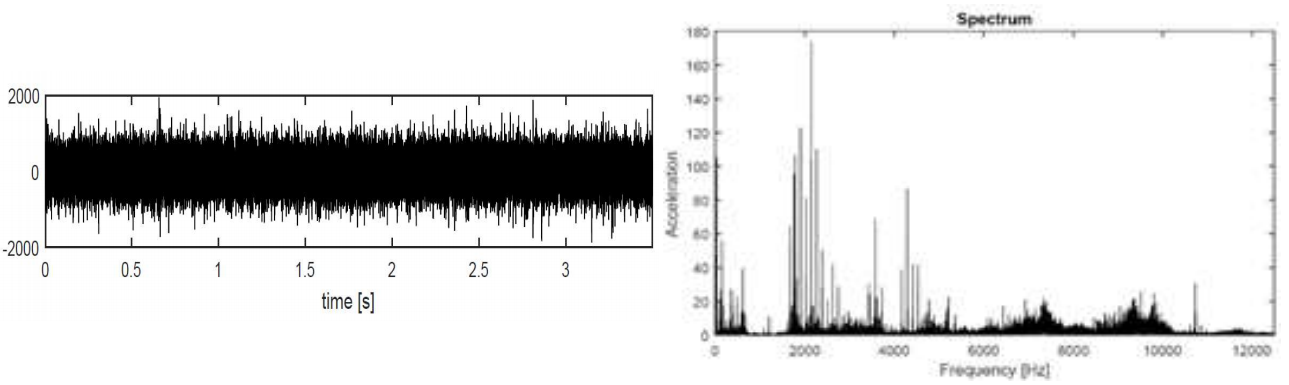
\includegraphics[width=0.75\linewidth]{ejkurtograma}
    			    \caption{Serie de tiempo (izquierda) y su espectro (derecha}
    			    \label{fig:ejkurtograma}
    			\end{figure}
    			Un pre-blanqueado de la señal y una posterior demodulación de la señal muestran resultados claros de una falla en la pista externa teniendo como resultado lo expuesto en la figura \ref{fig:ejkurtograma2}
    			\begin{figure}[H]
    			    \centering
    			    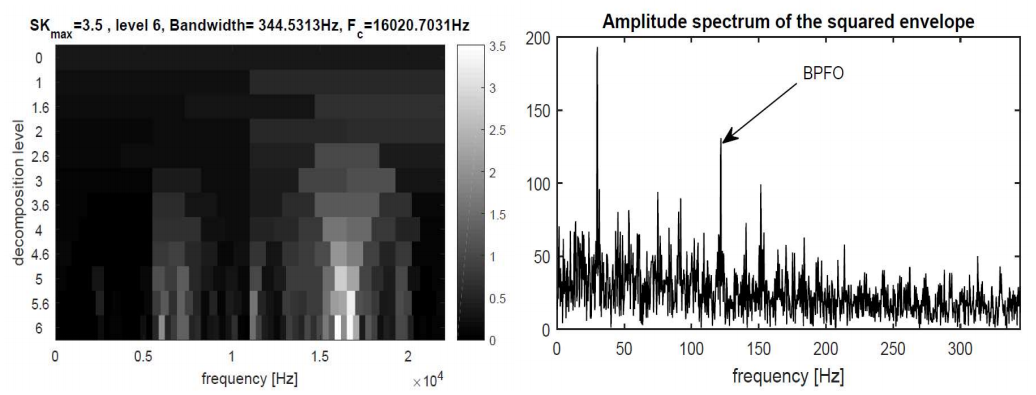
\includegraphics[width=0.75\linewidth]{ejkurtograma2}
    			    \caption{Aplicación curtograma (izquierda) y su demodulación (derecha)}
    			    \label{fig:ejkurtograma2}
    			\end{figure}
    			Del curtograma se ve que la frecuencia central de 16020 [Hz], con un ancho de frecuencias de 344.53 [Hz] posee el mayor valor de curtosis.
    \section{Mecanismos de Rotacion (Rotation Mechanism; RTM)}
        Los RTM son subsistemas dentro del sistema llamado \textit{Cúpula o Enclosure} (Figura \ref{fig:UTexteriorpartes}), los cuales son los encargados de soportar la cúpula y transmitirle el movimiento rotativo en ambos sentidos de giro, permitiendo así que en momentos de observación, la ventana de observación (OSD) gire en sincronía con el giro de azimut del telescopio teniendo una velocidad de operación (llamada tracking) de no mas de $0.03 \left[\frac{\circ}{sec}\right]$. y una velocidad de presetting de $2 \left[\frac{\circ}{sec}\right]$
        
        \begin{figure}[H]
            \centering
            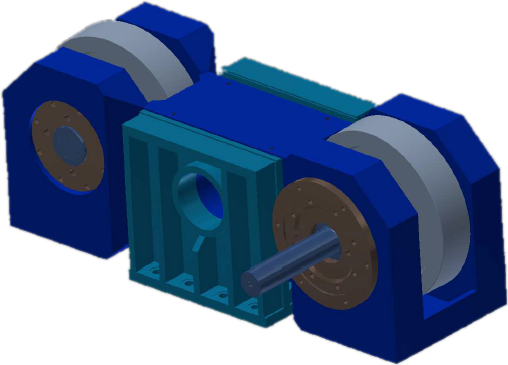
\includegraphics[width=0.5\linewidth]{RTMiso}
            \caption{Vista isometrica de un trolley del RTM}
            \label{fig:RTMiso}
        \end{figure}
        
        Cada telescopio cuenta con ocho unidades de RTM puestos equidistantes el uno con el otro los cuales soportan una carga total de $280.000 [Kg]$, lo que se traduce en $35000 [Kg]$ repartidos por RTM ó de $17.500 [Kg]$ por cada rueda. La ubicación física de estos equipos se encuentro en el nivel llamado \textit{Nasmyth} el cual se ubica aproximadamente a 11 metros del nivel \textit{G} o ground level (figura \ref{fig:topRTM}).
        \begin{figure}
            \centering
            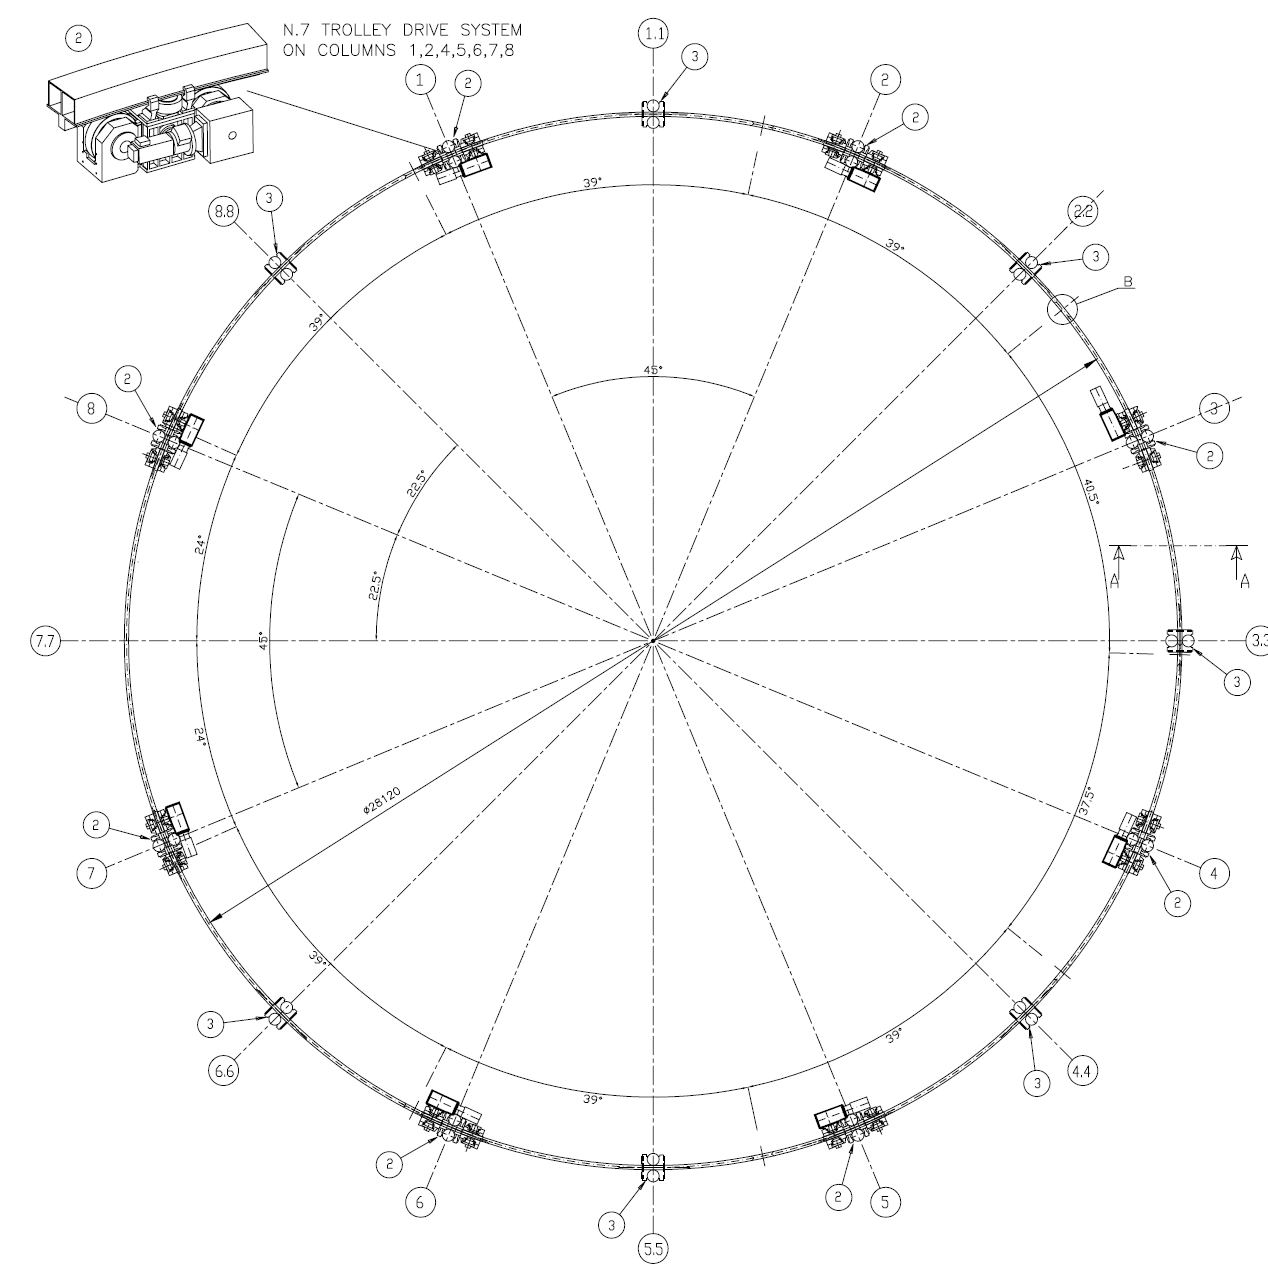
\includegraphics[width=\linewidth]{overviewRTM}
            \caption{Vista superior de RTM en nivel Nasmyth}
            \label{fig:topRTM}
        \end{figure}
            \subsection{Componentes de RTM}     
                \subsubsection{Carro del RTM}
                    Este subsistema es el mas importante de todos, este componente es en sí el cuerpo del RTM, el cual está montado en la parte central por una viga con un eje, el cual le permite al trolley actuar de balancín permitiendo una correcta distribución del peso de la cúpula en cualquier posición del movimiento de rotación (figura \ref{fig:RTMiso}).
                    
                    Este equipo esta constituido por dos ruedas montadas a cada extremo del trolley, una rueda conductora (conectada al motor/reductor) y una segunda rueda que tiene el eje conducido (o idle wheel)
                \subsubsection{Motor/Reductor}
                    La función principal de este componente es la transmisión del movimiento hacia una de las ruedas del RTM (Drive wheel o Rueda conducida), cada RTM funciona como un equipo independiente, es decir, cada uno cuenta con su propio motor/reductor. El motor marca \textit{Siemens} modelo \textit{FT5 106-OAA71-7} posee un torque nominal de $45 [Nm]$, el cual posee la capacidad de girar a diferentes frecuencias gracias al uso de un variador, este motor además posee un sistema de freno el cual tiene un torque: estático de 100 [Nm] y dinámico de 40[Nm] el cual permite frenar el enclosure (En caso de emergencia) en un tiempo menor a 5 [seg]
                    \begin{figure}[H]
        				\centering
        				\begin{subfigure}[b]{0.45\textwidth}
        					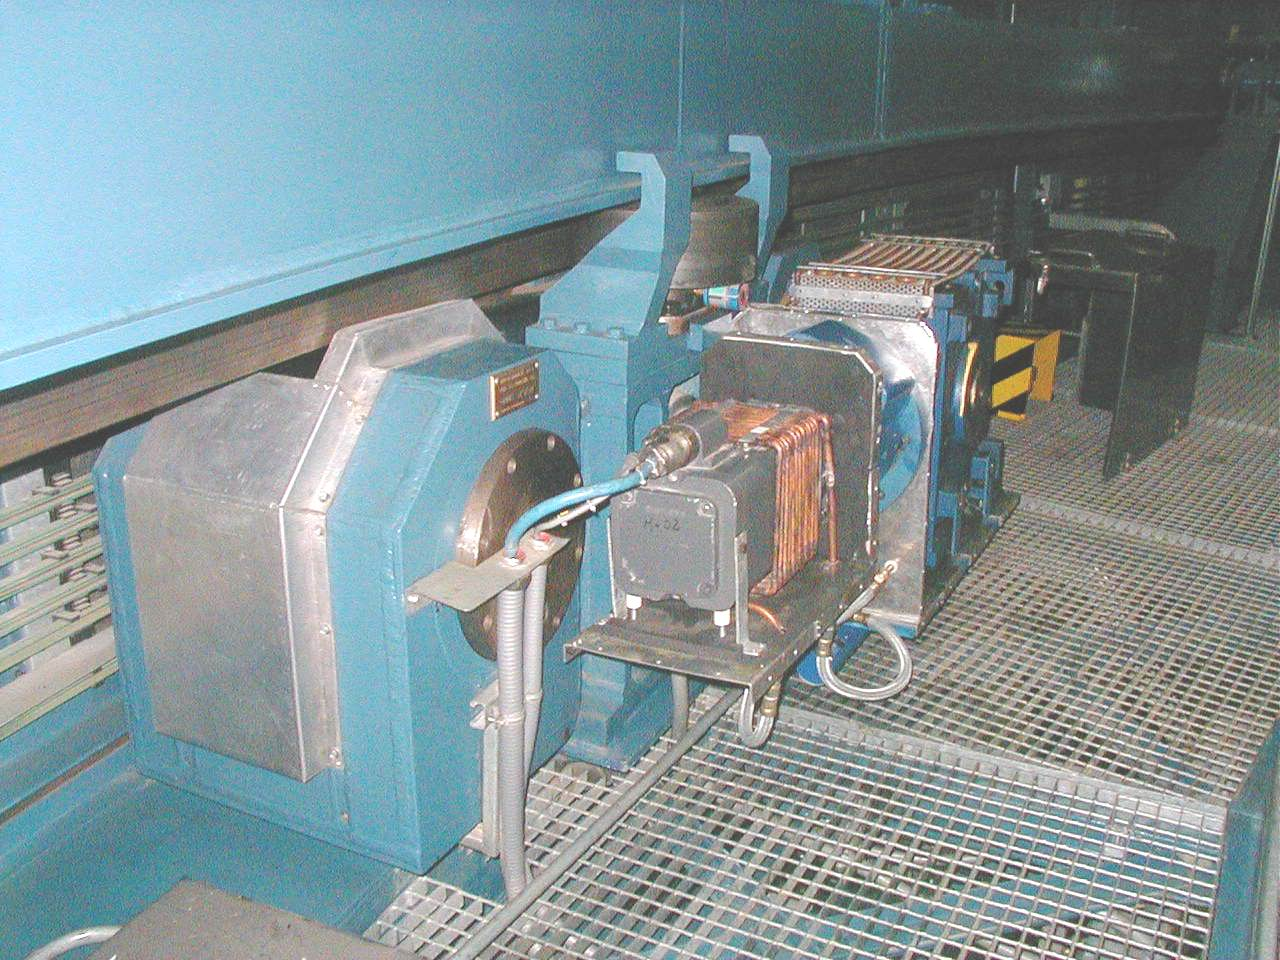
\includegraphics[width=\textwidth]{rtm_motor}
        					\caption{motor}
        					\label{fig:rtm_motor}
        				\end{subfigure}			    
        			    \begin{subfigure}[b]{0.45\textwidth}
        			    	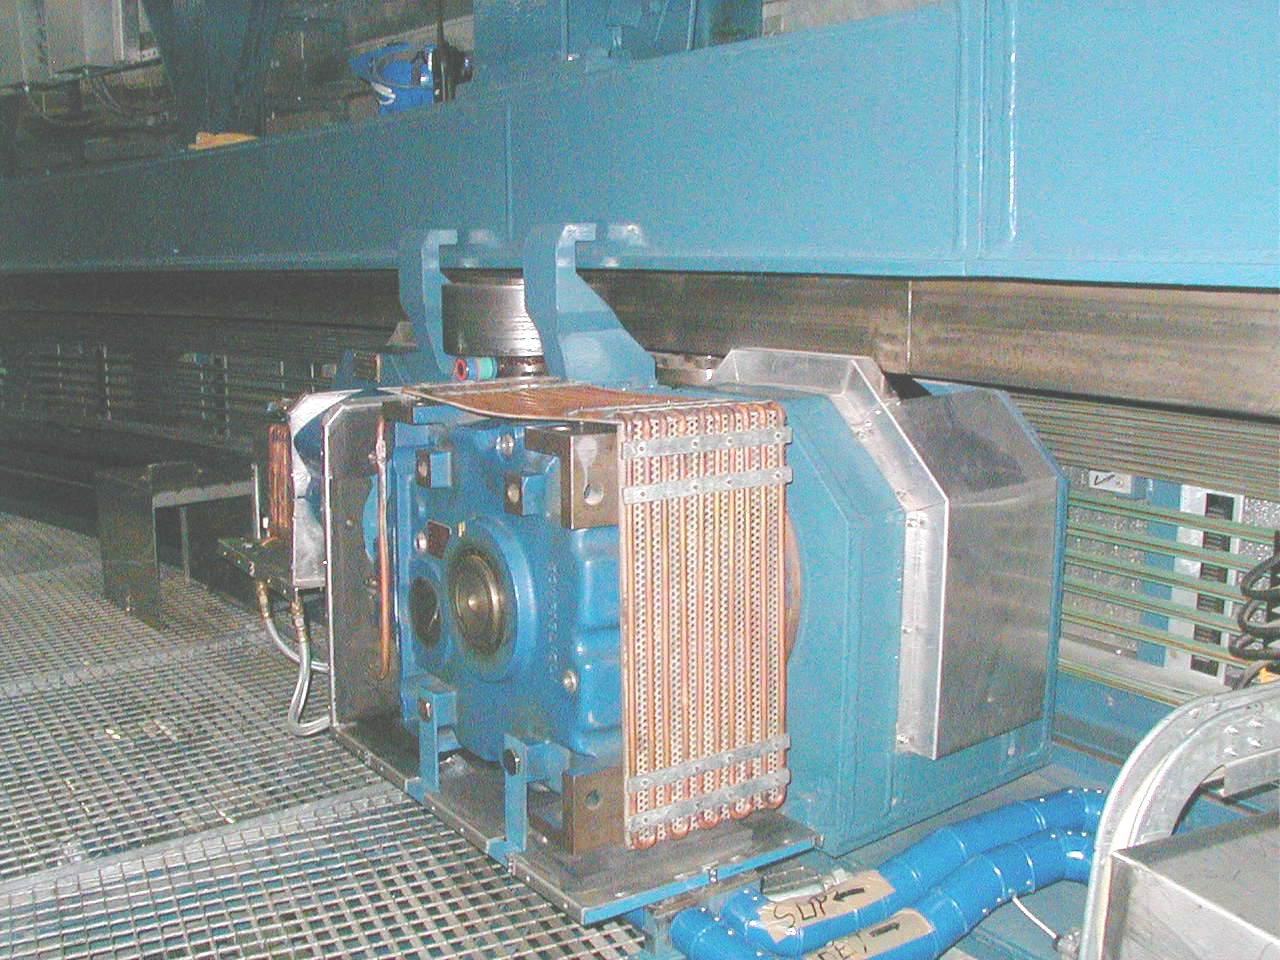
\includegraphics[width=\textwidth]{rtm_reductor}
        			    	\caption{reductor}
        			    	\label{fig:rtm_reductor}
        			    \end{subfigure}
        		        \caption{Componente motor/reductor de un RTM}
        		        \label{fig:rtm_motor_reductor}
                    \end{figure}
                    Sobre el reductor de velocidad, se encuentra una inconsistencia entre lo indicado por la hoja de calculo ( Doc.N$^{\circ}$: VLT-TRE-SEB-12300-0013 ) donde se indica que el reductor seleccionado posee un factor de reducción de $i=65.51$, al verificar la placa del equipo se nota que el reductor real seleccionado por la empresa diseñadora del sistema tiene un factor de reducción igual a 113.2 modelo RAO 90D C montaje tipo B8 modelo \textit{BONFIGLIOLI} (\href{http://www.brtspareparts.com/media/filer_public/be/4e/be4ee0b1-ac1a-4d38-9035-7b467686c8f4/br_strip_rao_1164_r0.pdf}{Link ficha técnica})
                \subsubsection{Acoplamiento flexible}
                    Este sistema, conecta el motor con el reductor. El acople elegido para unir ambos sistemas es del tipo flexible (figura \ref{fig:acople}) el cual actúa como elemento de seguridad o fusible mecánico. Cuando se genera un torque excesivo este acople se rompe haciendo que el motor se detenga de manera inmediata deteniendo al enclosure.
                    \begin{figure}
                        \centering
                        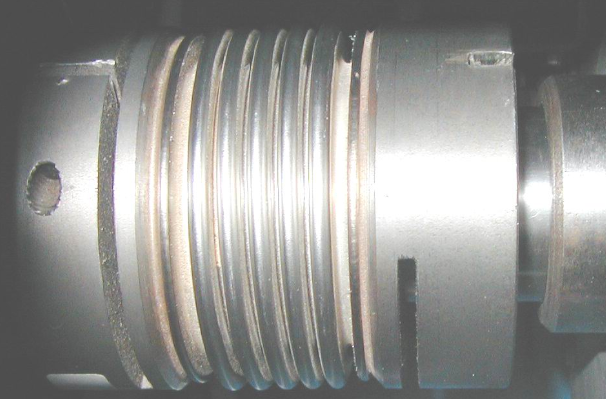
\includegraphics[width=0.5\linewidth]{acopleflexible}
                        \caption{Imágen del acople flexible}
                        \label{fig:acople}
                    \end{figure}
                \subsubsection{Patines Guías (Guide Rollers)}
                    Este mecanismo o subsistema permite que el enclosure mantenga su eje de giro, para eso cada RTM cuenta con dos ruedas guías (figura \ref{fig:topRTM},  \ref{fig:rtm_rollers}) junto con siete patines guías puestos de manera alternada entre RTM (figura \ref{fig:column_rollers}), además de las ruedas guías, el sistema cuenta con cuatro mordazas que actúan como tope mecánico en caso de falla de alguno de las ruedas laterales falle.
                    \begin{figure}[H]
        				\centering
        				\begin{subfigure}[b]{0.45\textwidth}
        					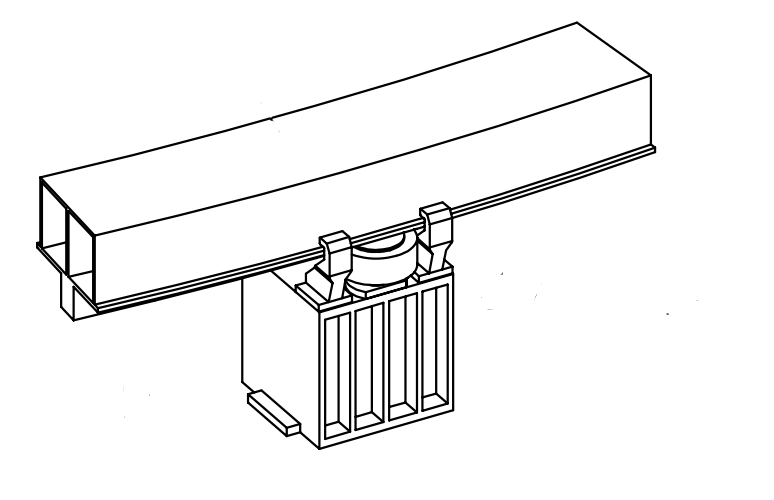
\includegraphics[width=\textwidth,height=5cm]{column_rollers}
        					\caption{Patines guías entre RTM}
        					\label{fig:column_rollers}
        				\end{subfigure}			    
        			    \begin{subfigure}[b]{0.45\textwidth}
        			    	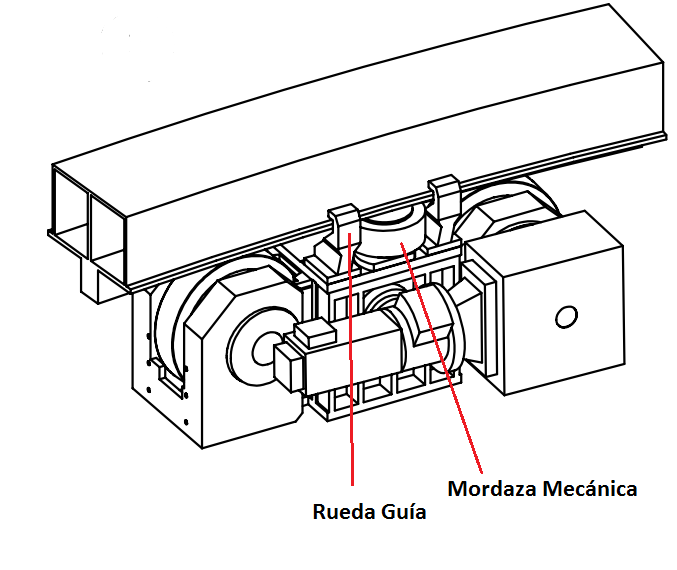
\includegraphics[width=\textwidth,height=5cm]{rtm_rollers}
        			    	\caption{Patines guías en RTM}
        			    	\label{fig:rtm_rollers}
        			    \end{subfigure}
        		        \caption{Dos tipos de patines guías en enclosure}
        		        \label{fig:rollers}
                    \end{figure}
                \subsubsection{Rodamientos}
                    Los rodamientos en los RTM son modelo SKF23030 del tipo esférico, cuentan con cuatro en total, dos por eje de ruedas. Sus especificaciones geométricas son:
                    \begin{figure}[H]
                        \centering
                        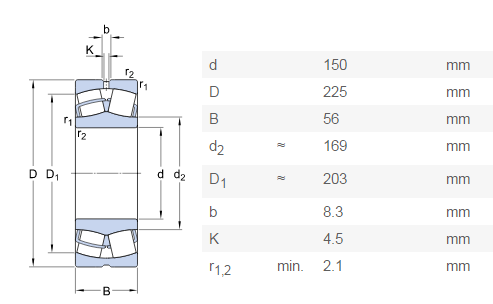
\includegraphics{rodamiento23030}
                        \caption{Dimensiones de rodamiento SKF23030}
                        \label{fig:rodamientoskf23030}
                    \end{figure}
                    
                    y sus tonos de rodamientos son:
                    
                    \begin{table}[H]
                        \centering
                        \caption{Tonos de rodamiento SKF23030}
                        \label{tab:tonosderodamiento}
                        \begin{tabular}{|c|c|}
                            \hline
                            \multicolumn{2}{c}{\begin{tabular}[c]{@{}c@{}}Bearing Frequencies {[}Hz{]}  \\ @8.2 RPM\end{tabular}} \\ \hline \hline
                            Velocidad Giro                                                & 0.137                                               \\ \hline
                            BPFI                                                          & 2.023                                               \\ \hline
                            BPFO                                                          & 1.667                                               \\ \hline
                            FTF                                                           & 0.062                                               \\ \hline
                            BSF                                                           & 0.695                                               \\ \hline
                            2*BSF                                                         & 1.391 \\ \hline                                    
                        \end{tabular}
                    \end{table}